\section{Implemented Mobility Protocol}
\label{app:concrete-protocol}

The following protocol instantiates the framework for the reported experiments. Its fixed target trips, daily rounds, route--departure actions, and link charges are implementation choices, rather than requirements on every future backend or study.

\subsection{Roles, Information, and Persistent State}
\label{sec:roles-state-implementation}

The road network is a directed graph $G=(V,E)$. Each simulated day $d=1,\ldots,D$ comprises full-day traffic execution and feedback. Agent identities, fixed attributes, experiences, summary memories, and active policies persist across days; vehicle movements are simulated anew.

LLM travelers control a fixed set of target trips, choosing routes and planned departure times. Target origins, destinations, modes, and candidate sets remain fixed. Their other trips and all trips by background travelers follow MATSim behavioral mechanisms, preserving full-day activity chains and replanning. An LLM pricing agent sets link charges; the archived implementation refers to this role as the manager. The roles interact through policies and shared traffic conditions, without direct exchanges of private information.

A traveler receives a synthetic profile, schedule references, candidate actions, static route information, recent personal outcomes, and a summary memory. Access to current toll announcements is fixed by person: informed travelers receive announcements relevant to their candidates; uninformed travelers learn from their own payments without observing the current policy. Past payments need not reflect current charges. Neither group receives network-wide real-time traffic information or realized travel times for unchosen routes. The comparisons below concern information supplied to controlled target decisions and their outcomes. Non-target trips retain background decision mechanisms and the same person-level announcement visibility assignment.

The manager receives public network information, aggregate traffic outcomes, policy history, and its own memory, excluding private traveler profiles and trip records. For each role, recent factual observations and a bounded LLM summary constitute the accessible history. The summary is replaced using the previous memory and new feedback; older experiences remain explicitly available only if retained in that summary. Full research archives are inaccessible to agents and distinguish environmental facts from generated interpretations.

\subsection{Travel and Management Actions}
\label{sec:actions-implementation}

For controlled target trip $i$, the traveler selects
\begin{equation}
    a_{i,d}=(r_{i,d},\tau_{i,d})\in\mathcal{R}_i\times\mathcal{T}_i,
    \label{eq:joint-action}
\end{equation}
where $\mathcal{R}_i$ and $\mathcal{T}_i$ are fixed route and departure-time sets. Routes satisfy network constraints, and departure times respect activity and simulation boundaries. The time grid is anchored to the original plan, rather than the previous day's choice. The LLM returns an action and a brief reason. Validity does not guarantee timely arrival or completion: preceding activities and trips can cause realized departure $\hat{\tau}_{i,d}$ to differ from selected departure $\tau_{i,d}$.

The manager periodically issues a complete policy assigning finite, nonnegative charges to eligible directed links. Unlisted links are free. The protocol limits the number of rules but imposes no preset price levels, upper price bound, or adjustment increment. If $p_d(e)$ is the charge per eligible entry to link $e$, target trip $i$ pays
\begin{equation}
    C_{i,d}=\sum_{n=1}^{N_{i,d}}p_d(e_{i,d,n}),
    \label{eq:realized-payment}
\end{equation}
where $e_{i,d,n}$ is the link entered at event $n$. Repeated entries incur repeated charges, and payments already incurred remain recorded for incomplete trips. Charges are constant within a day. For the same completed route and entry counts, changing departure time affects congestion and schedule outcomes but not the direct toll.

A valid policy replaces its predecessor; an empty policy removes all charges, and no update leaves the policy unchanged. The manager's task is to reduce full-day delay measured from completed link traversals. This measure differs from complete trip travel time, so evaluation also tracks completion, trip outcomes, and payments.

\subsection{Daily Execution and Feedback}
\label{sec:daily-cycle-implementation}

Each day follows a fixed sequence. First, the manager updates the policy when scheduled, using information available through day $d-1$. Travelers then choose actions from their permitted inputs. The simulator performs MATSim replanning, writes validated target actions into the plans, and executes all trips under the active policy. Individual outcomes and aggregate traffic summaries are returned to the respective roles, which update their memories for subsequent days. Travelers choose daily; the manager updates its memory daily and its policy periodically. The initial toll-free observation period also updates agent state.

Records distinguish selected actions, plan modifications, and realized execution, linking each to the relevant input, feedback, memory, and policy. These records support checks of action implementation and feedback timing. Failure handling and event bookkeeping are summarized in Appendix~\ref{app:implementation}.

\section{Demonstration Conditions}
\label{app:demonstration}
\label{sec:experimental-design}
\label{sec:scenario-conditions}

Table~\ref{tab:conditions} identifies the five recorded configurations. All use MATSim for traffic execution. MATSim agents select and replan activities and routes; constrained MNL and LLM travelers choose target actions within fixed candidate sets. Background trips retain MATSim mechanisms. The full set uses simulation seed 268 and paper days 1--100 (log Days~0--99). The archive labels \texttt{Native}, \texttt{Traveler}, \texttt{Manager}, and \texttt{Joint} correspond to MATSim, LLM Traveler, MATSim + Pricing, and LLM Traveler + Pricing, respectively. Population and information assignments use seed 6021; the fixed target cohort spans 2,877 OD pairs.



Management update opportunities occur on paper days 21, 51, and 81 after a 20-day toll-free period. MATSim + Pricing begins positive charging on day 21; LLM Traveler + Pricing retains zero charges until day 51, then charges links \texttt{43\_3} and \texttt{43\_4} at 1.5 scenario units per entry and retains these charges on day 81. The combined configuration assigns 5,897 travelers to current toll announcements and 5,896 to no current announcements, with personal feedback available to both groups.

Input checks cover network, population, facilities, capacities, target identities, and background settings. Candidate-based configurations share fixed route and departure options; MATSim agents are not restricted to those options. Matching inputs does not remove differences in executable builds, preference representations, or remote model responses. The MNL baseline uses uncalibrated homogeneous coefficients. Definitions and settings appear in the following appendices.
\FloatBarrier

% Technical appendix fragment. Insert after \appendix; do not add a document class.
% Packages: amsmath, array, booktabs, tabularx, placeins, hyperref.
% Sources: completed100 analysis reports and archived manifest_snapshots.json.
% Prompt descriptions below are summaries, not reconstructed original prompts.

\section{Scenario, Candidate Actions, and Configuration}
\label{app:configuration}

\subsection{Population and Target Selection}

The input scenario contains 84,110 people. Sampling sorts person identifiers, shuffles them with Java Random using seed 6021, and retains a fixed 20\% subset with all its plans, yielding 16,822 simulated travelers. Network flow and storage capacity factors are 0.2 and $0.2^{0.75}\approx0.2991$, respectively \cite{mersiniScalingMATSimTraffic2026,ben-dorPopulationDownscalingMultiagent2021}. Population sampling, synthetic profiles, information groups, and controlled-roster selection use seed 6021; the main simulation seed is 268.

Targets are selected from original plans using destination-activity start times in $[0,32400)$ seconds, corresponding to starts before 09:00. Selection covers all activity purposes and requires one car leg per target trip; it imposes no departure-window filter. Missing or invalid planned arrival times are excluded rather than imputed. The selected cohort contains 11,793 trips by 11,793 people across 2,877 OD pairs. Membership remains fixed throughout the experiment. The remaining 5,029 people and non-target trips of controlled people retain MATSim decision mechanisms. Work-arrival evaluation uses the fixed subset of 11,332 targets with work deadlines. The 09:00 selection threshold does not substitute for each trip's deadline.

\subsection{Fixed Candidate Sets}

Runs reuse the same precomputed BFS-LE candidate file \cite{rieser2013route}, validating topology, costs, overlap, and the shortest-route candidate without regenerating or reordering alternatives. The archived settings specify up to four candidates per OD pair and maximum pairwise overlap 0.85. For free-flow time, an alternative passes the detour check if its ratio to the reference is at most 2.5 or its excess time is at most 300 seconds. The analogous distance limits are 2.5 and 2,000 meters; both time and distance checks must pass. The exact overlap implementation and original candidate-file hash belong to the reproducibility archive.

Departure candidates span $-5400$ to $+1800$ seconds relative to the original planned departure, at 900-second intervals. Options are clipped against the original origin-activity start, day zero, and the exclusive simulation end; the original departure is retained. The arrival deadline is not a hard feasibility filter. Subsequent choices do not shift the original time anchor. Of the targets, 2,780 have one route and 9,013 have multiple routes; the former cannot contribute route switches within the fixed candidate space.

\begin{table}[htbp]
\centering\small
\caption{Principal archived settings for the 100-day experiment. Strategy weights are configuration weights, not probabilities inferred from their sum.}
\label{tab:configuration}
\renewcommand{\arraystretch}{1.15}
\begin{tabularx}{\linewidth}{@{}>{\raggedright\arraybackslash}p{0.35\linewidth}X@{}}
\toprule
Setting & Value \\
\midrule
MATSim version & 2026.0 \\
Population / simulation seeds & 6021 / 268 \\
Initial strategy weights & \texttt{ChangeExpBeta}: 0.7; \texttt{ReRoute}: 0.1; \texttt{TimeAllocationMutator}: 0.1 \\
Innovation cutoff & Log Day90, equivalent to paper day 91; existing-plan selection continues \\
Simulation interval for charging & $[0,108000)$ seconds \\
Manager opportunities & Paper days 21, 51, and 81 \\
Toll action limits & At most 40 distinct car links; finite nonnegative charge per entry; no preset price cap or increment \\
Recent personal observations & Up to three preceding days \\
Personal summary limit & 500 characters \\
Manager summary limit & 1,000 English words; target length 400--600 words, with no enforced minimum \\
Information groups & 5,897 informed and 5,896 uninformed; fixed person-level assignment \\
\bottomrule
\end{tabularx}
\end{table}

The effective innovation cutoff is established from the run logs and final configuration, rather than inferred solely from the initial strategy entries. Both background replanning and MATSim-agent target decisions are affected; LLM and MNL target choices continue under their respective decision mechanisms.

\section{Implementation, Information, and Execution Protocol}
\label{app:implementation}

This appendix describes how the current implementation
coordinates agent decisions, environmental execution,
and persistent states. It supplements the interaction
framework with implementation-specific information rules,
memory updates, output validation, and event bookkeeping.

\subsection{Implementation Components and Data Flows}
\label{app:implementation-components}

Figure~\ref{fig:implementation_dataflow} summarizes the
logical components of the current implementation.
The coordinator constructs role-specific inputs, schedules
decision and memory tasks, and validates generated outputs.
The execution adapter applies accepted choices and policies
in MATSim and extracts the outcomes needed for personal
and public feedback.

Agent-accessible histories and summaries support subsequent
decisions, while the research archive preserves linked
records for inspection. These components represent logical
responsibilities rather than separate deployed services.
The implementation distinguishes generated requests,
accepted actions, and realized outcomes throughout this
process.

\begin{figure}[!tbp]
    \centering
    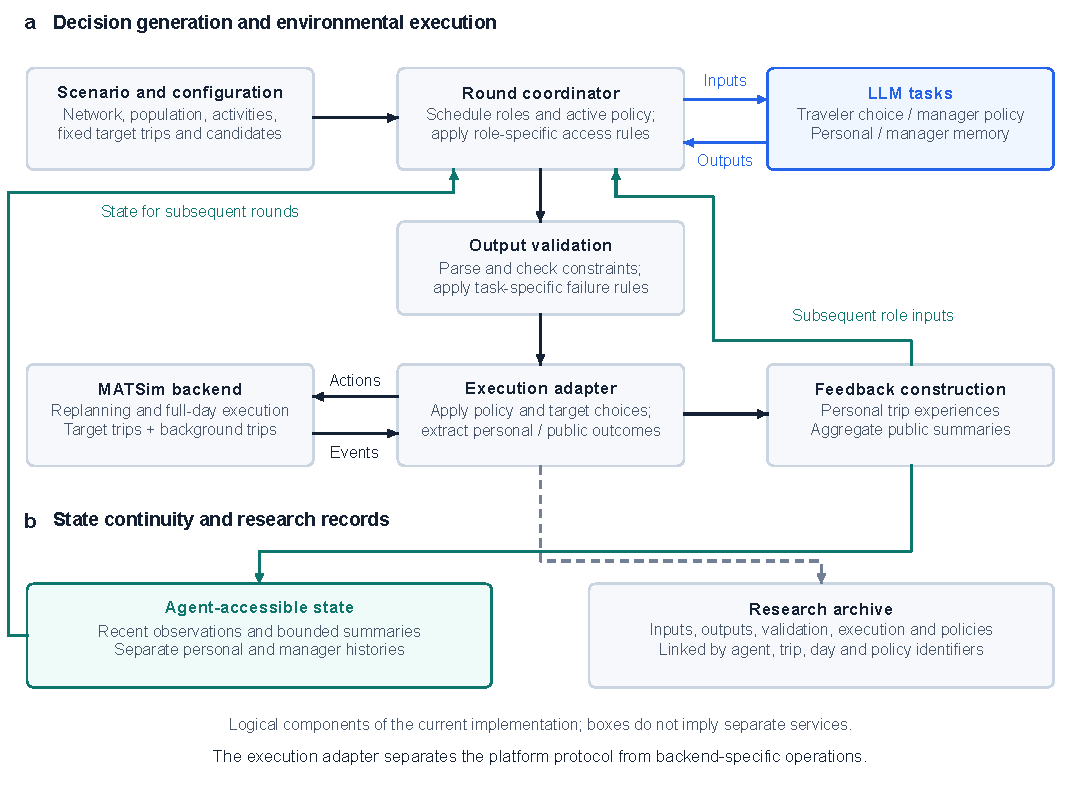
\includegraphics[width=\linewidth]
        {sections/pic/fig_implementation_dataflow.pdf}
    \caption{Logical components and data flows in the
    current implementation.
    (a) Role-specific inputs and generated outputs pass
    through coordination and validation before accepted
    actions are applied through the execution adapter.
    Returned events support personal and aggregate feedback.
    (b) Agent-accessible states support subsequent decisions,
    while a separate archive retains research records.
    Dashed arrows denote research-record linkage.}
    \label{fig:implementation_dataflow}
\end{figure}

\subsection{Information Access and Initialization}
\label{app:information-access}

Announcement visibility is assigned at person level:
all trips of a controlled person share the same visibility
assignment. The LLM selects actions only for the designated
target trip; other trips retain background routing and
time-adjustment mechanisms. For uninformed people, current
toll information remains unknown, although background
routing can retain personal link/time-bin observations.
People outside the treatment use the background
information mechanism.

Informed target decisions receive current toll estimates
for their candidate actions. Uninformed decisions receive
null current costs rather than zero costs. Both groups
receive static candidate information, recent personal
outcomes, and their own summaries, without network-wide
realized traffic conditions or outcomes for unchosen routes.
The LLM Traveler configuration explicitly communicates
that charging is disabled. In the combined configuration,
informed and uninformed inputs remain distinct even when
the active policy is empty.

Initial factual histories and self-written summaries are
empty. Synthetic profiles specify assumed preferences;
they do not represent observed past experiences.

The manager receives public network information, aggregate
reference-plan OD diagnostics, completion statistics,
aggregate link traffic, and its own policy and memory
histories. Private traveler profiles, memories, and
individual payments are excluded. The archived manager
projection retains the latest two executed policy-version
effects and pools older days, with aggregate recent/previous
statistics over windows of up to seven days. All-car links
remain represented in the public network, while detailed
traffic projection prioritizes high-delay or failed links
and currently or recently charged links. This projection
is distinct from the travelers' three-day personal window.

\subsection{Experience Retention and Memory Updates}
\label{app:memory-updates}

Figure~\ref{fig:memory_update} distinguishes recent factual
observations, generated summaries, and research records.
For each controlled traveler, completed-trip outcomes enter
a rolling personal history covering up to three preceding
days. A separate LLM task generates a replacement summary
from the previous memory and newly available feedback.
After validation, the new summary fully replaces the
previous one.

Personal histories and summaries remain associated with
the person and target trip and are not shared across agents.
No separate exact-payment history is available to the LLM
outside its bounded observations and summary. Once an
outcome leaves the recent-history window, its influence
through explicit historical context depends on what the
summary retains. The research archive preserves full
records for inspection but does not provide unrestricted
retrieval memory to agents.

Manager memory is updated after each completed day,
including toll-free days, independently of scheduled
policy decisions. Its inputs use public feedback and
the manager's own history. A memory update does not
change the active policy.

\begin{figure}[!tbp]
    \centering
    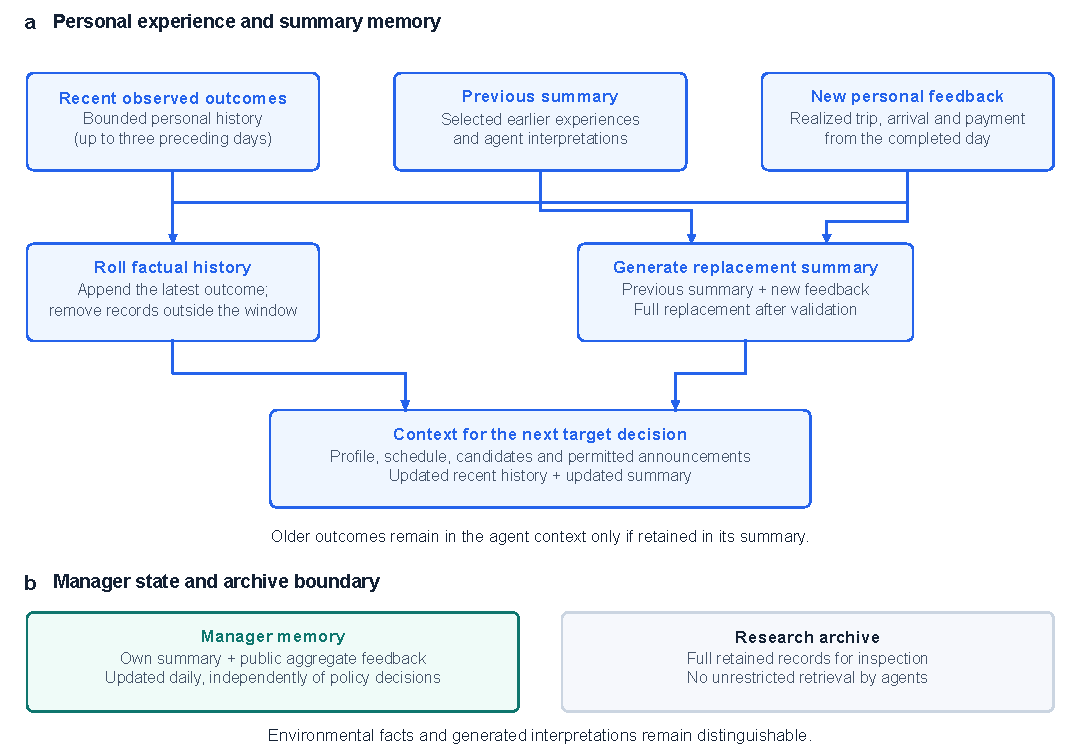
\includegraphics[width=\linewidth]
        {sections/pic/fig_memory_update.pdf}
    \caption{Experience retention and memory updates.
    (a) New personal feedback updates the rolling factual
    history and supplies a separate summary-generation task.
    The updated history and validated replacement summary
    enter subsequent target-decision contexts.
    (b) Manager memory is updated daily from public feedback,
    independently of policy decisions. Research archives
    remain separate from agent-accessible histories.}
    \label{fig:memory_update}
\end{figure}

\subsection{Output Validation and Failure Handling}
\label{app:output-validation}

Figure~\ref{fig:validation_failure} summarizes the validation
stages and task-specific failure rules. Traveler outputs
are checked for exact JSON, permitted route and departure
values, and configured character limits. Each task permits
at most three output attempts: the initial attempt and
up to two retries. Truncated responses are rejected without
salvaging partial JSON or inventing actions. Persistent
traveler-decision or personal-memory failure terminates
the experiment rather than silently substituting a stale
summary.

Failed or invalid manager-memory updates retain the
previous memory. The next successful update includes
the missing days. Manager-policy failures follow the
configured policy-failure protocol; detailed retry,
fallback, and transport-error handling must be interpreted
with the archived implementation. Output-repair counts
alone do not characterize these paths.

Structured-output validation does not establish semantic
accuracy. References to unavailable route identifiers
within summary text are logged diagnostically rather than
automatically rewritten. Semantic review was disabled in
the reported runs, so syntactic validity does not certify
the factual correctness of summaries or the faithfulness
of generated reasons. Late arrival and noncompletion are
environmental outcomes, not automatically output-format
failures.

\begin{figure}[!tbp]
    \centering
    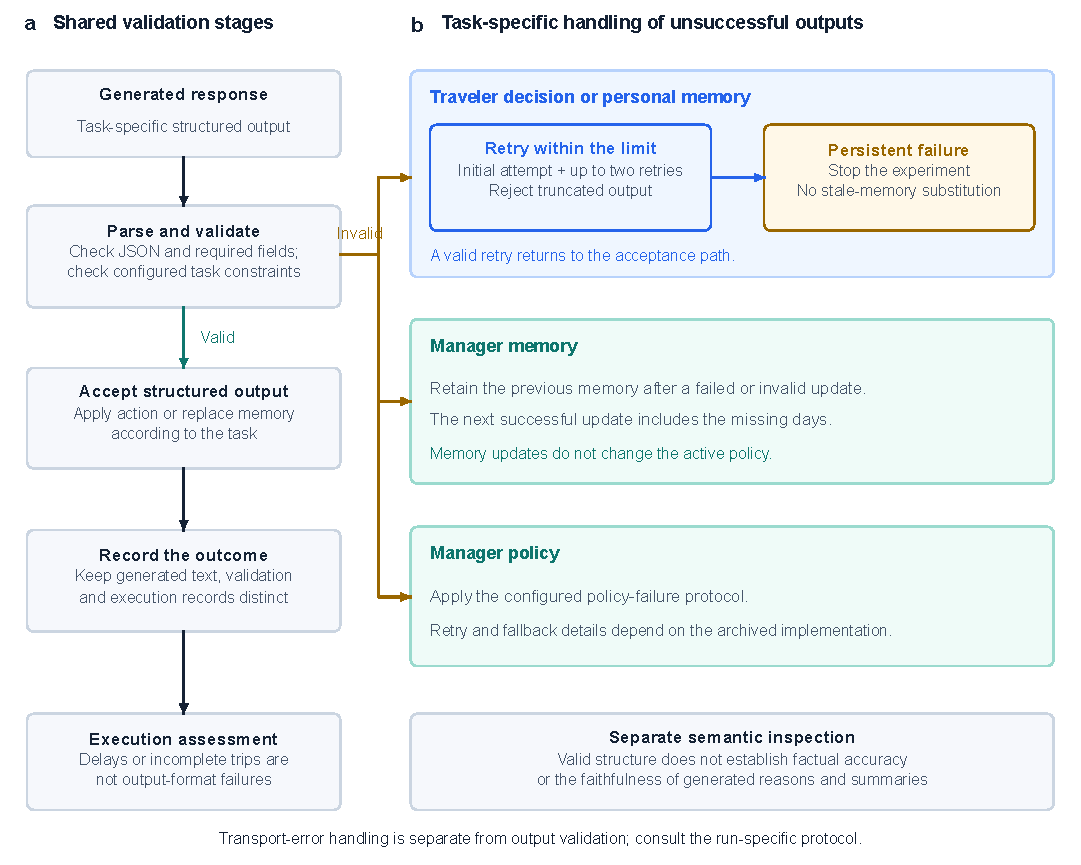
\includegraphics[width=\linewidth]
        {sections/pic/fig_validation_failure.pdf}
    \caption{Output validation and task-specific failure
    handling.
    (a) Structured outputs are checked before acceptance,
    with validation and execution recorded separately.
    (b) Persistent traveler-task failure stops the experiment;
    failed manager-memory updates retain the previous state.
    Manager-policy failures follow the configured protocol.
    Transport-error handling and semantic assessment remain
    separate from structured-output validation.}
    \label{fig:validation_failure}
\end{figure}

\subsection{Plan Execution and Billing}
\label{app:execution-billing}

Scheduled manager decisions precede environmental execution.
MATSim replanning is followed by writing validated route
and departure choices into the controlled target plans.
Other selected-plan activity ends are retained.
Original, selected, and realized departure times are
stored separately because preceding activities, queues,
and earlier trips can delay execution.

Tolls are charged on eligible car-link entries, including
the origin partial link under the archived billing
convention. Repeated traversals incur repeated charges,
while duplicate notifications of the same entry are
ignored. Charges apply over the half-open interval
$[0,108000)$ seconds and remain constant within a day.
Payments already incurred are retained if a trip
subsequently fails to complete. Candidate cost estimates
and actual payments are recorded separately.

A valid policy replaces the entire rule set, and an empty
policy removes all charges. Policy episodes are identified
by effective prices; a new version with unchanged prices
does not constitute a new price intervention.
Link-delay statistics use completed full-link traversals
and therefore have different event boundaries from toll
collection and trip-duration measurement.

\section{Measurement and Aggregation}
\label{app:measurement}

\paragraph{Choice changes and collective redistribution.}
Behavioral measures use selected actions, with realized departure times retained separately. Let $\mathcal{I}$ be the fixed cohort of $N=11{,}793$ targets and $\rho_{i,d}$ the complete ordered link sequence of the selected route. Population-wide rates are
\begin{equation}
 R_d=\frac{1}{N}\sum_{i\in\mathcal{I}}\mathbf{1}(\rho_{i,d}\ne\rho_{i,d-1}),
 \qquad
 A_d=\frac{1}{N}\sum_{i\in\mathcal{I}}\mathbf{1}(\tau_{i,d}\ne\tau_{i,d-1}),
 \label{eq:behavioral-adjustments}
\end{equation}
for paper days $d=2,\ldots,100$, corresponding to log transitions ending on Days~1--99. All targets have valid actions in these transitions. Candidate-based multi-route rates restrict both numerator and denominator to 9,013 targets; the remaining 2,780 cannot switch within their fixed route sets. MATSim agents are not restricted to those sets. A route is identified by its full link sequence, not its local candidate label. Aggregate route-flow turnover is $\sum_{o,r}|n_{o,r,d}-n_{o,r,d-1}|/(2N)$, where $n_{o,r,d}$ counts targets by OD pair $o$ and complete route $r$. Offsetting individual switches need not alter these counts.

Mean daily car time per person is calculated as
\[
\bar{T}^{\mathrm{car}}_d
=
\frac{60 T^{\mathrm{car}}_d}{16{,}822},
\]
where $T^{\mathrm{car}}_d$ is total daily car time in
person-hours. The normalized measure is reported in
minutes per person for each simulated day.

\paragraph{Time, schedule, and payment outcomes.}
Total daily car time sums car-departure-to-car-arrival durations across the population, including waiting before network entry. A complete total is undefined if a planned car trip is incomplete. Target-time distributions use completed target trips; completion and work-arrival measures retain their original cohort denominators. For 11,332 work targets, on-time completion, late completion, and noncompletion exhaust the cohort. All planned car trips completed in the reported runs.

Selected departure offsets are measured relative to original plans, and the earliest-option share counts selections of the earliest available candidate. Mean early arrival averages $\max(\mathrm{deadline}-\mathrm{arrival},0)$ over all work targets, including zeros. Mean daily P95 averages each day's target-time 95th percentile; individual savings compare each person's mean time over the common window. No monetary value is assigned to early arrival or departure inconvenience. Target payments and full-day personal payments use different trip scopes.

\paragraph{Aggregation and comparison windows.}
All five runs contribute paper days 1--100 (log Days~0--99). Outcome summaries average daily values over that window; relative changes are ratios of window means minus one, and lateness differences are percentage points. Choice-change rates average 99 adjacent-day transitions. Cutoff diagnostics treat log Day~90 separately and use Days~91--99 for the post-cutoff window. Plotted smoothing uses a trailing seven-day mean. Successive days and travelers within a shared run do not provide independent run-level replications.

Link-delay comparisons first aggregate original link records to full days to reconcile reporting intervals. Completed-link delay excludes waiting before network entry. Target/other-trip and waiting/post-entry decompositions each recover total car time and are alternative accounts of the same total.

\section{Execution Audit and Computational Workload}
\label{app:audit-cost}

Output repair was required for 2,433 finalized travel-decision records (0.206\%) and 2,943 personal-memory records (0.250\%). All personal memory chains were continuous, submitted memories remained within 500 characters, and no finalized travel decision was blank. The three management decisions were valid; one invalid management-memory JSON response was repaired through retry, with all 100 daily updates completed. These checks establish consistency of accepted outputs and state updates, without implying that every initial generation was valid or that generated reasons and memories were semantically correct.

\begin{table}[htbp]
\centering
\small
\caption{Recorded LLM inference workload over complete 100-day runs. Counts include retries and repairs across roles; tokens are service-reported totals. Zero LLM calls does not imply zero simulation cost.}
\label{tab:cost}
\begin{tabularx}{\linewidth}{@{}Xrr@{}}
\toprule
Condition & API calls & Tokens \\
\midrule
MATSim & 0 & 0 \\
MNL & 0 & 0 \\
LLM Traveler & 2,362,964 & 5,713,538,990 \\
MATSim + Pricing & 109 & 872,774 \\
LLM Traveler + Pricing & 2,364,090 & 5,451,720,152 \\
\bottomrule
\end{tabularx}
\end{table}

The combined run contains 1,181,736 traveler-decision calls, 1,182,250 personal-memory calls, three management-decision calls, and 101 management-memory calls. There are 1,179,300 finalized records for each personal task. The excess calls include repair and retry overhead and cannot be interpreted as hallucination counts. Logged tokens do not measure monetary cost, GPU energy, or end-to-end runtime. Semantic correctness of all memories and faithfulness of generated reasons have not been systematically established.

\section{Archived Demonstration Outputs}
\label{app:supplementary}

Tables~\ref{tab:validation-outcomes} and~\ref{tab:supp-switching} record selected outputs from one run per configuration at seed 268. They describe outputs of the recorded configurations and support the illustrative uses in Section~\ref{sec:illustrative-use}; their rankings are not estimates of general comparative effectiveness or robustness. Repeated days and person-days are dependent observations. Rounding limits display precision; it does not quantify uncertainty. Full-precision aggregate data are retained in the accompanying 100-day documentation package.

\begin{table}[htbp]
    \centering
    \small
    \caption{Archived output summaries over the common 100-day window (traffic seed 268). Entries are daily means, rounded for display; rankings apply only to these recorded runs. Total car time includes all car trips and waiting before network entry; work lateness uses the fixed denominator of 11,332 trips. These are summaries of one run per configuration, not independent-replication estimates.}
    \label{tab:validation-outcomes}
    \renewcommand{\arraystretch}{1.15}
    \begin{tabularx}{\linewidth}{@{}>{\raggedright\arraybackslash}X r r r@{}}
        \toprule
        Condition & \shortstack{Total car time\\(person-h/day)} & \shortstack{Target time\\(min/trip)} & \shortstack{Work lateness\\(\%)} \\
        \midrule
        MATSim & 12,431 & 29.3 & 20.0 \\
        MNL & 17,201 & 53.2 & 31.3 \\
        LLM Traveler & 9,958 & 17.4 & 5.6 \\
        MATSim + Pricing & 12,663 & 29.6 & 20.4 \\
        LLM Traveler + Pricing & 11,414 & 16.3 & 3.7 \\
        \bottomrule
    \end{tabularx}
\end{table}

\begin{table}[htbp]
\centering\small
\caption{Mean daily choice-change rates over 99 adjacent-day transitions. Overall rates use 11,793 targets; multi-route rates use 9,013 eligible targets. A dash denotes a candidate-space comparison that is not applicable. All entries are percentages.}
\label{tab:supp-switching}
\begin{tabularx}{\linewidth}{@{}Xrrr@{}}
\toprule
Condition & \shortstack{Overall\\route changes} & \shortstack{Multi-route\\changes} & \shortstack{Departure\\changes} \\
\midrule
MATSim & 5.26 & --- & 20.05 \\
MNL & 48.55 & 63.52 & 85.24 \\
LLM Traveler & 3.08 & 4.03 & 29.45 \\
MATSim + Pricing & 5.43 & --- & 20.28 \\
LLM Traveler + Pricing & 2.19 & 2.86 & 28.04 \\
\bottomrule
\end{tabularx}
\end{table}

A supplementary MATSim--pricing pair at seed 9261 is retained in the archive. It is not a replication of the five-condition experiment or the information-group comparison. Its presence does not change the single-run scope of the tables above.

\subsection{Run-Specific Reproduction Artifacts}
\label{app:archive-scope}

The analysis archive preserves effective configurations, input and executable hashes, candidate sets, accepted actions, attempts, experiences, policy histories, and memory updates. The distribution documentation supplies aggregate CSVs and audit summaries. A run-specific reproduction bundle must additionally identify the corresponding code revision or executable, original prompt templates, model-service settings, and input versions. Public access locations and the mapping from release artifacts to historical builds should accompany that bundle; the scope supported by the current documentation is described in Section~\ref{sec:reproducibility}.
% AUTHOR CHECK: Supply verified immutable release/run identifiers and accessible
% raw-artifact locations before claiming exact historical regeneration.
\FloatBarrier
